\documentclass[openany, 12pt]{book}

\usepackage{UNCCHDissertation}

\title{CALIOPE, A Search for CP Violation in Positronium
}
\author{Chelsea Lynn Bartram}
\advisor{Reyco Henning}
\committee{\advisorname, John Wilkerson, Jonathan Heckman, Jonathan Engel, Art Champagne, David C. Radford}
\theyear{2015}

\begin{document}

\frontmatter

% Make the titlepage
\maketitlepage

% Make the copyright page
\makecopyrightpage

% Abstract (350 word limit)
\begin{abstract}
  We propose to search for CP-violation in the charged lepton sector by studying ortho-positronium decays.
  Positronium, a bound state of an electron and positron, occurs in both a singlet and triplet state. The triplet
  state, ortho-positronium, decays primarily into three gamma rays. CP-violation could potentially manifest
  itself in angular correlations between the directions of the three photons and the spin of the ortho-positronium
  (o-Ps). We propose to use the APEX annular array of NaI detectors for gamma ray detection, combined
  with a tagged source and a novel, conventional electromagnet. APEX will increase the angular acceptance,
  hence, statistics, by a factor of 25 over previous experiments. We also implement several experimental
  improvements to reduce our systematic uncertainties compared to previous experiments. I will present
  the current status of the experiment, named CALIOPE, which stands for CP Aberrant Leptons in Ortho-
  Positronium Experiment, and our future plans.

\end{abstract}

\begin{acknowledgements}
  I would like to thank my parents, Lynn and Peter Bartram, and sister, Chloe Bartram. Additionally, I would like to thank Janice Yong, my college roommate and best friend, for her unwavering support and invaluable outsider perspective. Furthermore, I owe it to my physics friends from BU, who, even though we separated for grad school, have continued to support each other. 
  This is dedicated to James F. Bartram, my grandfather and electrical engineer, and Jeremiah Lynch, my grand-uncle, an industrial hygenist. They set the bar so high both in the sciences and as kind, conscientious human beings. 
  Thanks also goes out to my group members Joule Othman and undergraduates.
  Thanks to Reyco Henning.
  Finally, I would like to dedicate this to Karen Thompson, my friend and pancreatic cancer survivor for 12 years, who taught me the true meaning of gratitude, forgiveness, and how to be optimistic against all odds. You helped me re-frame my graduate school experience and gave me the strength to never give up.
\end{acknowledgements}

% Make table of contents
\maketableofcontents

% Make a list of tables
\maketablelist

% Make a list of figures
\makefigurelist

% List of symbols and abbreviations
\begin{AbbrevList}
    \item[$0\nu\beta\beta$] Neutrinoless Double-beta Decay
    \item[$2\nu\beta\beta$] Double-beta Decay 
	\item[BEGe] Broad Energy Germanium
    \item[C.L.] Confidence Level
    \item[CMB] Cosmic Microwave Background
    \item[DFSZ] Dine, Fischler, Srednicki, and Zhitnitsky Axion Model 
    \item[DSWT] Discrete Stationary Wavelet Transform
    \item[DWT] Discrete Wavelet Transform
    \item[GAT] Germanium Analysis Toolkit
	\item[HPGe] High Purity Germanium
    \item[KSVZ] Kim, Shifman, Vainstein, and Zakharov Axion Model
	\item[KURF] Kimballton Underground Research Facility
	\item[MALBEK] \textsc{Majorana} Low-background BEGe Detector at Kimballton
    \item[pdf] Probability Distribution Function
    \item[PEP] Pauli Exclusion Principle
	\item[PPC] P-type Point Contact
    \item[$Q$] End-point Energy
    \item[ROI] Region of Interest
    \item[SBC] Single Board Computer
    \item[SIS3302] Struck Innovativ Systeme 3302 Digitizer
    \item[SURF] Sanford Underground Research Laboratory
	\item[WIMP] Weakly Interacting Massive Particle
    \item[WMAP] Wilkinson Microwave Anisotropy Probe
\end{AbbrevList}

\mainmatter

%=====================%
\chapter{Introduction}
%=====================%
%-------------------------------------------------------------------%
\section{Fundamental Symmetries}
%-------------------------------------------------------------------%

Fundamental symmetries provide a mechanism for understanding the world. There are three discrete fundamental symmteries. Their respective operators are C, which stands for ``Charge'', P, which stands for ``Parity'', and T, which stands for ``Time''. For a long time it was assumed that these symmetries were absolutely conserved. Indeed, they are quite intuitive. This worldview was disrupted when partiy violation was first discovered by CS Wu. Paritry symmetry went unquestioned until 1956 when T.D. Lee and C.N. Yang postulated its possibility and noticed evidence for its existence was gravely lacking~\cite{PhysRev.104.254}. C.S. Wu demonstrated the existence of partiy violation with her famous cobalt-60 experiment, in which electrons from beta decay were emitted in a preferential direction relative to the spin orientation of the cobalt nuclei~\cite{PhysRev.105.1413}. Parity was violated an violated maximally. The effect was substantial. Nevertheless, deep-seated assumptions about symmetries, perhaps based on instinct, were hard to displace. The belief that combinations of symmetry operators must be valid symmetries persisted. The union of charge and partity, or CP symmetry was the next tenet to be challenged when in 1964, Cronin and Fitch discovered CP violation in the decay of kaons ~\cite{PhysRevLett.13.138}. The discovery of CP violation has since prompted physicists to search for other symmtery violating effects, resulting in the discovery of CP violation in both D and B meson oscillations ~\cite{PhysRevLett.87.091801}.
Discoveries of symmetry violations actually provide an explanation for other cosmological phenomena. In 1967, Andrei Sakharov pointed ou that CP violation is necessary to explain the existing baryon asymmetry in the universe ~\cite{0038-5670-34-5-A08}. These are the so-called Sakharov conditions and they must have manifested themselves in the early universe in order to produce the matter-antimatter asymmetry. Though numerous examples of symmetry violations have been found, the combination of all three symmetry operators, CPT, is generally believed to be a conserved symmetry. CP-violation has only been observed in the weak interactions of the quark sector. Its existence in the lepton sector has not been confirmed experimentally. Notably, long-baseline neutrino experiments are being constructed at great cost to look for CP-violation in the neutrinos. Experiments such as DUNE (Deep Underground Neutrino Experiment) require a baseline which runs from Illinois to South Dakota and a collaboration of more than 525 scientists and engineers~\cite{LBNE}. Other groups have been searching for CP-violation in the charged lepton sector as well. For example, if the electron has an electric dipole moment, this would be a sign of T violation, which is equivalent to CP-violation, provided CPT is conserved ~\cite{PhysRevLett.100.120801}.


%-------------------------------------------------------------------%
\section{Another Section}
\label{sec:mjd}


Our experiment will search for CP-violation in positronium. Positronium consists of two charged leptons: an
electron and positron. Unlike experiments such as DUNE, however, our experiment occupies much less space,
costs orders of magnitude less, and employs only a few people. CALIOPE is a table-top nuclear experiment
which will be assembled at TUNL, the Triangle Universities Nuclear Laboratory. Specically, we propose to
search for CP-violating angular correlations between the three gamma rays emitted from ortho-positronium
decay and the spin of the positronium. Such CP-violating correlations are predicted within the Standard
Model, but at levels far below our detection limit

\section{Previous Experiments}
\label{sec:mjd}
Previous experiments studying the angular correlations in ortho-positronium decay did not observe any CPviolation.
The rst measurement was made by M. Skalsey and J.V. House in 1991 [10]. This experiment
found no CP amplitude at the 1:5% level. In 2010, Yamazaki, Namba, Asai, and Kobayashi measured an
amplitude of a CP-violating asymmetry consistent with zero at a sensitivity of 2:10􀀀3 [9]. This result
was a factor of 7 improvement in the limit from the previous experiment. Our experiment will use an array
with much greater angular coverage, increasing our statistics by a factor of 25. In addition, we will be
implementing several features to improve systematic uncertainties over previous experiments. These are
described below. Although it is hard to tell what our ultimate sensitivity improvement will be over previous
experiments, we can conservatively estimate it to be a factor of 10 or more.2
%-------------------------------------------------------------------%

\section{Theory of Positronium}
Positronium was first discovered by Martin Deutsch at MIT in 1951 [11]. He was able to show that the time
it took for gamma rays emitted from the positronium source to reach the detector was longer than would be
expected from ordinary annihilation, implying the existence of a long-lived bound state.
Positronium's energy levels can be obtained by modeling it like the hydrogen atom but replacing the
mass of the proton with the reduced mass of the electron and positron. Unlike the hydrogen atom, however,
positronium is unstable and decays into gamma rays after a nite amount of time. Like the hydrogen atom,
positronium also comes in both a triplet (S = 1) and singlet (S = 0) state. For this experiment, we are only
concerned with positronium in its ground state where n = 1.
The number of gamma rays emitted is determined by charge conjugation invariance. Charge conjugation
parity in positronium is given as C = (􀀀1)s+l, where s is the spin quantum number and l is the orbital
angular momentum number. In our system, positronium decays from the l = 0 state, so the C parity is
􀀀1 for the triplet state and 1 for the singlet state. C parity is multiplicative, and the photon has odd
charge conjugation parity. Therefore, the triplet state, also known as ortho-positronium, decays into three
photons with odd charge conjugation parity and the singlet state, or para-positronium, decays into two
photons with even charge conjugation parity. While it is possible for ortho-positronium to decay into a
larger, odd number of photons (and likewise, para-positronium into a larger, even number of photons), this
rarely happens because the branching ratios for these decays are greatly suppressed.
Number of photons aside, the triplet state and singlet state can also be easily dierentiated by their
lifetimes. The triple state has a much smaller phase space and an extra vertex that contributes an extra
factor of the ne structure constant. These two features extend the lifetime of the triplet state (142 ns) to
nearly a factor of 1000 greater than that of the singlet state (125 ps).



\subsection{$CP$-Violating Correlation}

 $CP$-violation in ortho-positronium decay could manifest itself as a $CP$-violating angular distributions of the emitted gamma rays. One such $CP$-violating correlation, as introduced by Bernreuther~\cite{Bernreuther:1981ah}, can be written in the following way:

 \begin{align}
 \Braket{\vec{S}{\cdot}\vec{n}}
 \end{align}

 $\vec{S}$ is the spin polarization axis and $\vec{n}$ is the normal to the ortho-positronium decay plane. A measurement of this alone would not only be conclusive of $CP$-violation, but also of $CPT$-violation. Though this would be an interesting experimental search, it is not the focus of our proposal.

 In our experiment, which searches for $CP$-violation exclusively, we measure the following correlation, which is $CPT$-conserving:

 \begin{align}
 Q=P_{2}(\vec{S}{\cdot}\vec{k_{1}})(\vec{S}{\cdot}\vec{k_{1}}{\times}\vec{k_{2}})=P_{2}\sin{2\theta}\sin{\psi}\cos{\phi}
 \end{align}

Here, $\vec{S}$ is the spin of the ortho-positronium, and $\vec{k_{i}}$ is the direction of the $i^{th}$ most energetic gamma ray from the decay. $P_{2}$ is known as the tensor polarization. $\theta$ is the angle between the normal to the ortho-positronium decay plane and the spin quantization axis. $\phi$ is the angle between $\vec{k_{1}}$ and the projection of the spin quantization axis onto the ortho-positronium decay plane. $\psi$ is the angle between the $\vec{k_{1}}$ and $\vec{k_{2}}$ vectors (See Figure 1). 

 \begin{figure}[H]
 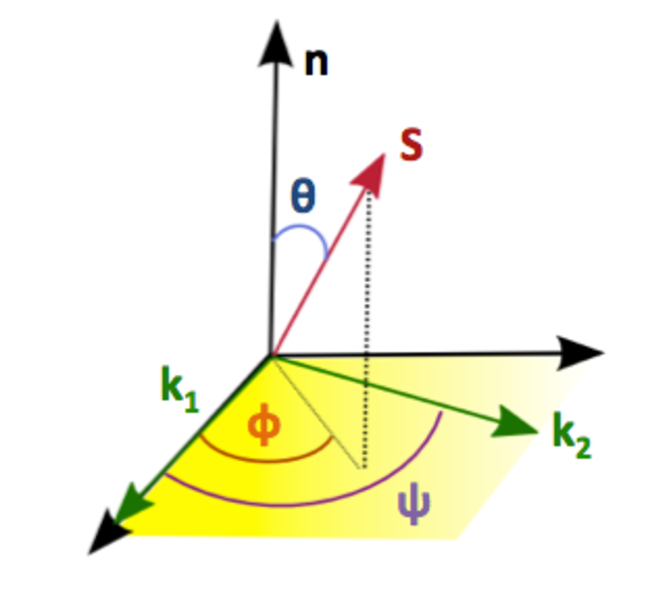
\includegraphics[width=0.4\textwidth,center]{spinAngles.pdf}
 \caption{o-Ps Angles}
 \end{figure}

 This term, $Q$, is sometimes called the \emph{analyzing power}~\cite{PhysRevLett.104.083401}, which is scaled by the $CP$-violating amplitude in the decay rate.
 \begin{align}
 N=N_{0}[1+C_{CP}\left(\vec{S}{\cdot}\vec{k_{1}}\right)\left(\vec{S}{\cdot}\vec{k_{1}}{\times}{\vec{k_{2}}}\right)]
 \end{align}

We will measure the following asymmetry term:
\begin{align}
A=C_{CP}Q(\theta,\psi,\phi)
\end{align}

A positronium system with non-zero asymmetry exhibits $CP$-violation.

The tensor polarization (also known as spin-alignment term), $P_{2}$, is defined as follows:
 \begin{align}
 P_{2}=\frac{N_{+1}-2N_{0}+N_{-1}}{N_{+1}+N_{0}+N_{-1}}=0
 \end{align}
$N_{m}$ stands for the number of o-Ps in the $m^{th}$ quantum state, where $m$ is the $m_{s}$ quantum number of ortho-positronium. With no magnetic field present, these states have the same half-life and are equally populated at all times, yielding $P_{2}=0$. An external magnetic field mixes the triplet $m=0$ state with the singlet state and shortens its half-life, yielding a nonzero value for $P_{2}$ that is time-dependent. The $m={\pm}1$ states are unaffected by the external B-field.

 The magnitude of this effect is dependent upon the magnetic field strength. Generally speaking, the greater the magnetic field, the greater the mixing (Figure 2). When $P_{2}$ is nonzero, we are able to look for $CP$-violation, as the analyzing power would then have nonzero amplitude.


 \begin{figure}[H]
 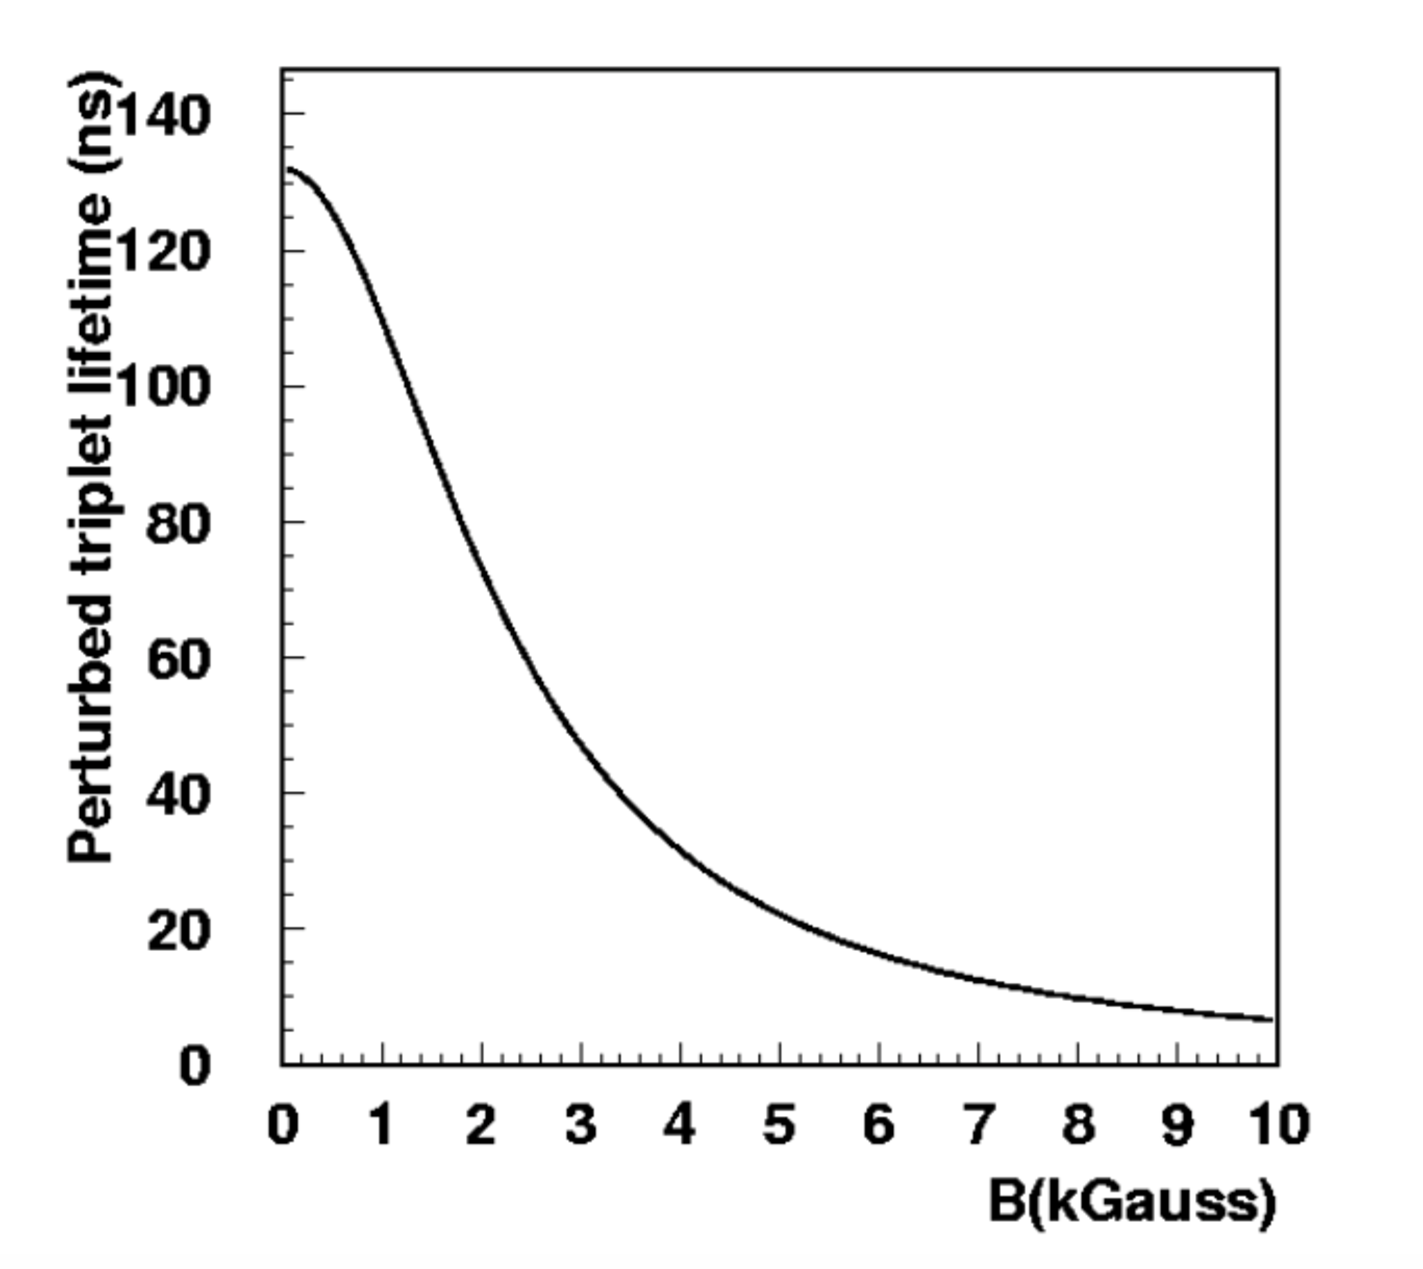
\includegraphics[width=0.45\textwidth,center]{Lifetime_BField.pdf}
 \caption{Ortho-positronium lifetime in a magnetic field (in vacuum)~\cite{Felcini:2004yn}}
 \end{figure}

 The energies and momenta of the gamma rays must abide by the usual conservation laws, where $m$ is the rest mass of the electron and $\vec{k_{i}}$ are the momenta vectors of the gamma rays:

 \begin{align}
 {\lvert}\vec{k_{1}}{\rvert}+{\lvert}\vec{k_{2}}{\rvert}+{\lvert}\vec{k_{3}}{\rvert}&=2m \\
 \vec{k_{1}}+\vec{k_{2}}+\vec{k_{3}}&=\vec{0} 
 \end{align}

 The energy spectra is given by the following equation, where $m$ is the rest mass of the electron, as derived by Ore and Powell~\cite{PhysRev.75.1696}:

 \begin{align}
 F(k_{1})&={\int}^{m}_{m-k_{1}}\left(\frac{m^2(m-k_{1})^2}{k_{2}^2k_{3}^2}+\frac{m^2(m-k_{2})^2}{k_{3}^2k_{1}^2}+\frac{m^{2}(m-k_{3})^2}{k_{1}^{2}k_{2}^{2}}\right)\frac{dk_{2}}{m} \\
 &=2\left(\frac{k_{1}(m-k_{1})}{(2m-k_{1})^{2}}-\frac{2m(m-k_{1})^{2}}{(2m-k_{1})^{3}}\ln\left(\frac{m-k_{1}}{m}\right)+\frac{2m-k_{1}}{k_{1}}+\frac{2m(m-k_{1})}{k_{1}^{2}}\ln\left(\frac{m-k_{1}}{m}\right)\right)
 \end{align}

Due to the symmetry in the distributions, we can use this equation to pick values for the two highest energy photons when we perform Monte Carlo simulations, for example. The energy for $\vec{k_{3}}$ is determined by conservation of energy. Figures 3 and 4 show the $\vec{k_{1}}$ and $\vec{k_{2}}$ energy distributions, respectively.

\begin{figure}[!htb]
  \centering
     \begin{minipage}{0.5\textwidth}
         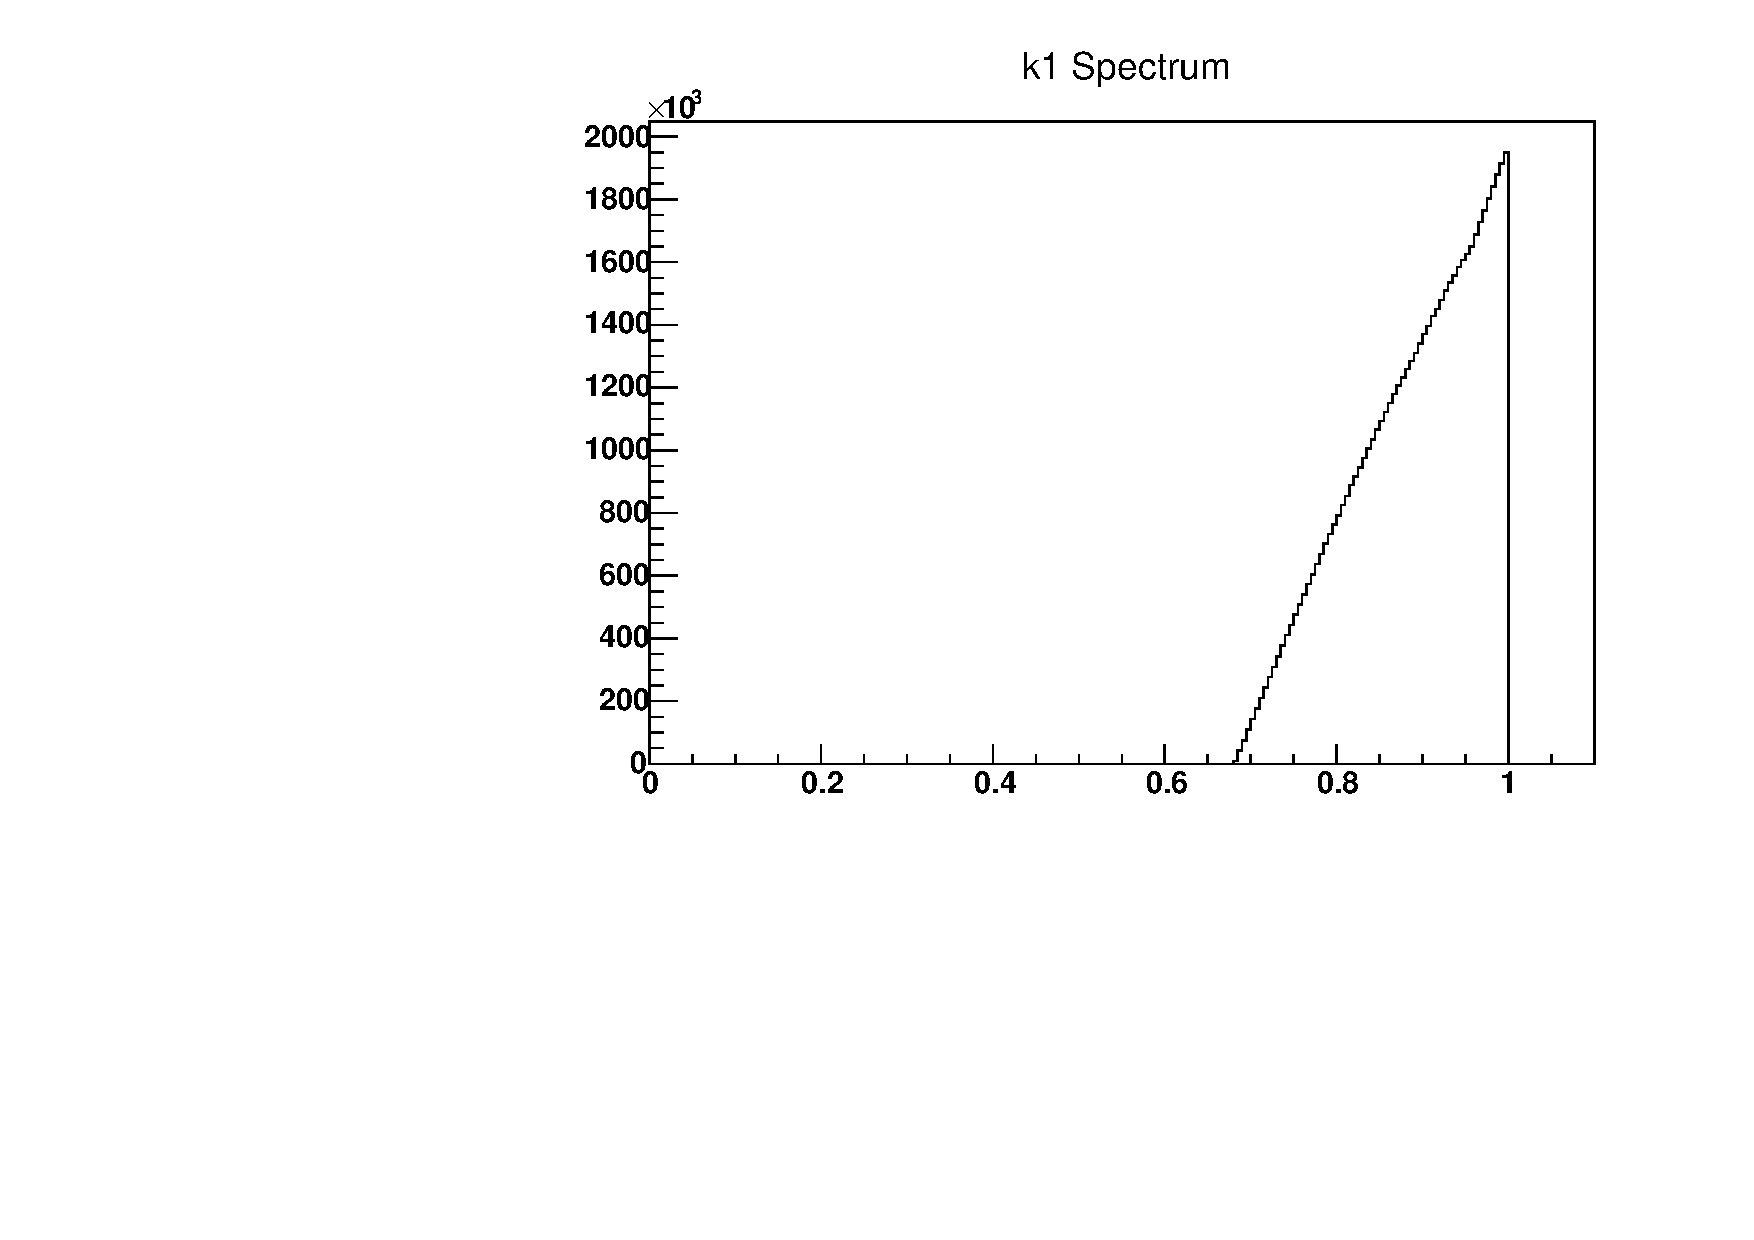
\includegraphics[width=1.0\linewidth]{k1Spectrum.pdf}
         \caption{$k_{1}$ Energy Spectrum}
     \end{minipage}%                                                                                                                        
     \centering
     \begin{minipage}{0.5\textwidth}
         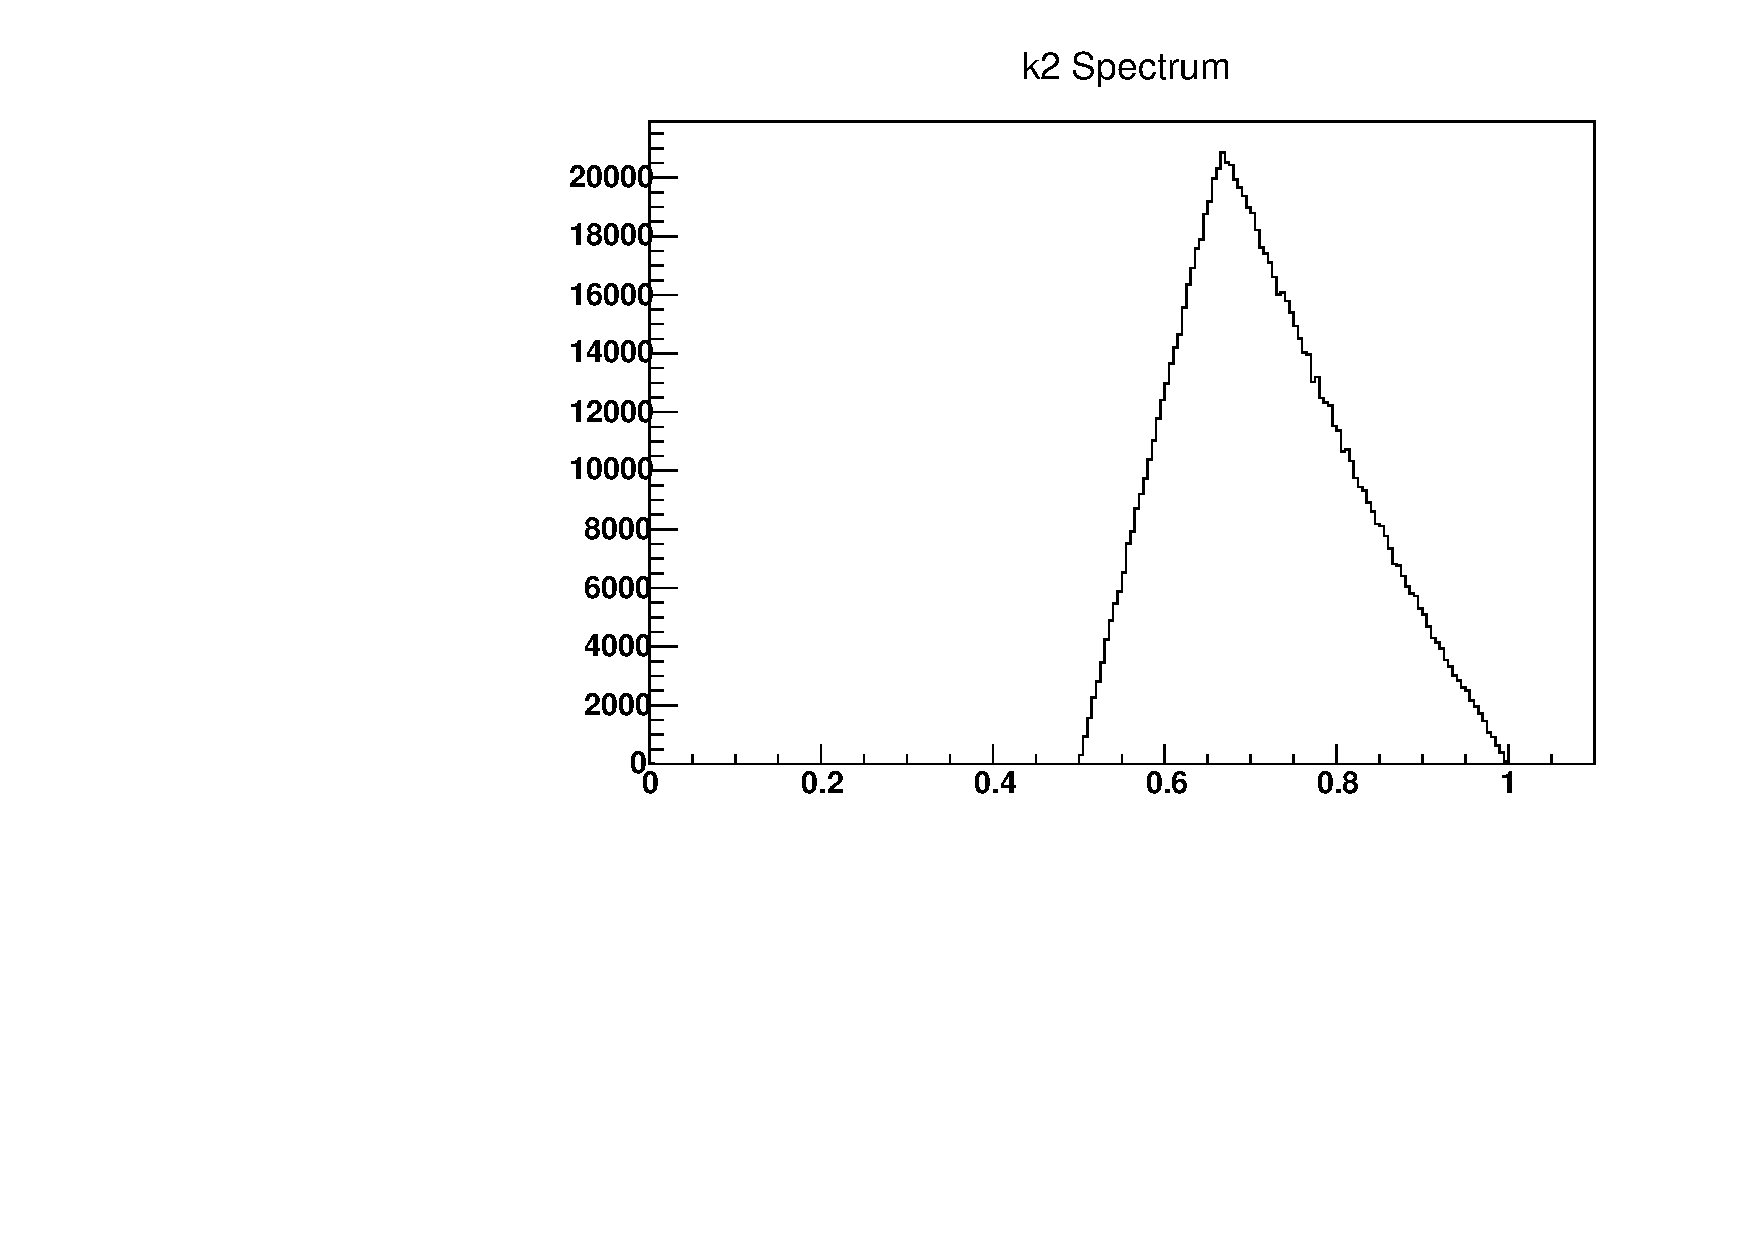
\includegraphics[width=1.0\linewidth]{k2Spectrum.pdf}
         \caption{$k_{2}$ Energy Spectrum}
     \end{minipage}
\end{figure}


 In the presence of $CP$-violation, the energy spectrum for the small fraction of $CP$-violating decays will depend on the physics of the $CP$-violating process, which is unknown. For our work we will use a simple model that only includes basic phase space considerations, as computed by Ore and Powell. It is easy to check different models using Monte Carlo simulations in the future.

The Standard Model predicts an angular distribution for the gamma rays emitted in ortho-positronium. This distribution was determined by Bernreuther~\cite{Bernreuther:1981ah} and changes depending on the magnetic quantum number  of the ortho-positronium. For $m=0$ states, the angle, $\theta$, which is defined as the angle between the normal to the decay plane and the spin, the distribution is given as $P(\theta)=1+{\cos}^{2}\theta$. For $m={\pm}1$, the distribution is given as $P(\theta)=\frac{3-{\cos}^2{\theta}}{2}$.

In conclusion, positronium is a well-understood leptonic system, not complicated by effects from quarks and QCD. It serves as a probe for fundamental symmetries, in particular for searches for $CP$-violation.

 \vspace{5mm}


% ------------  figure start  
% from M. Busch
\begin{figure}[htbp]
\centering
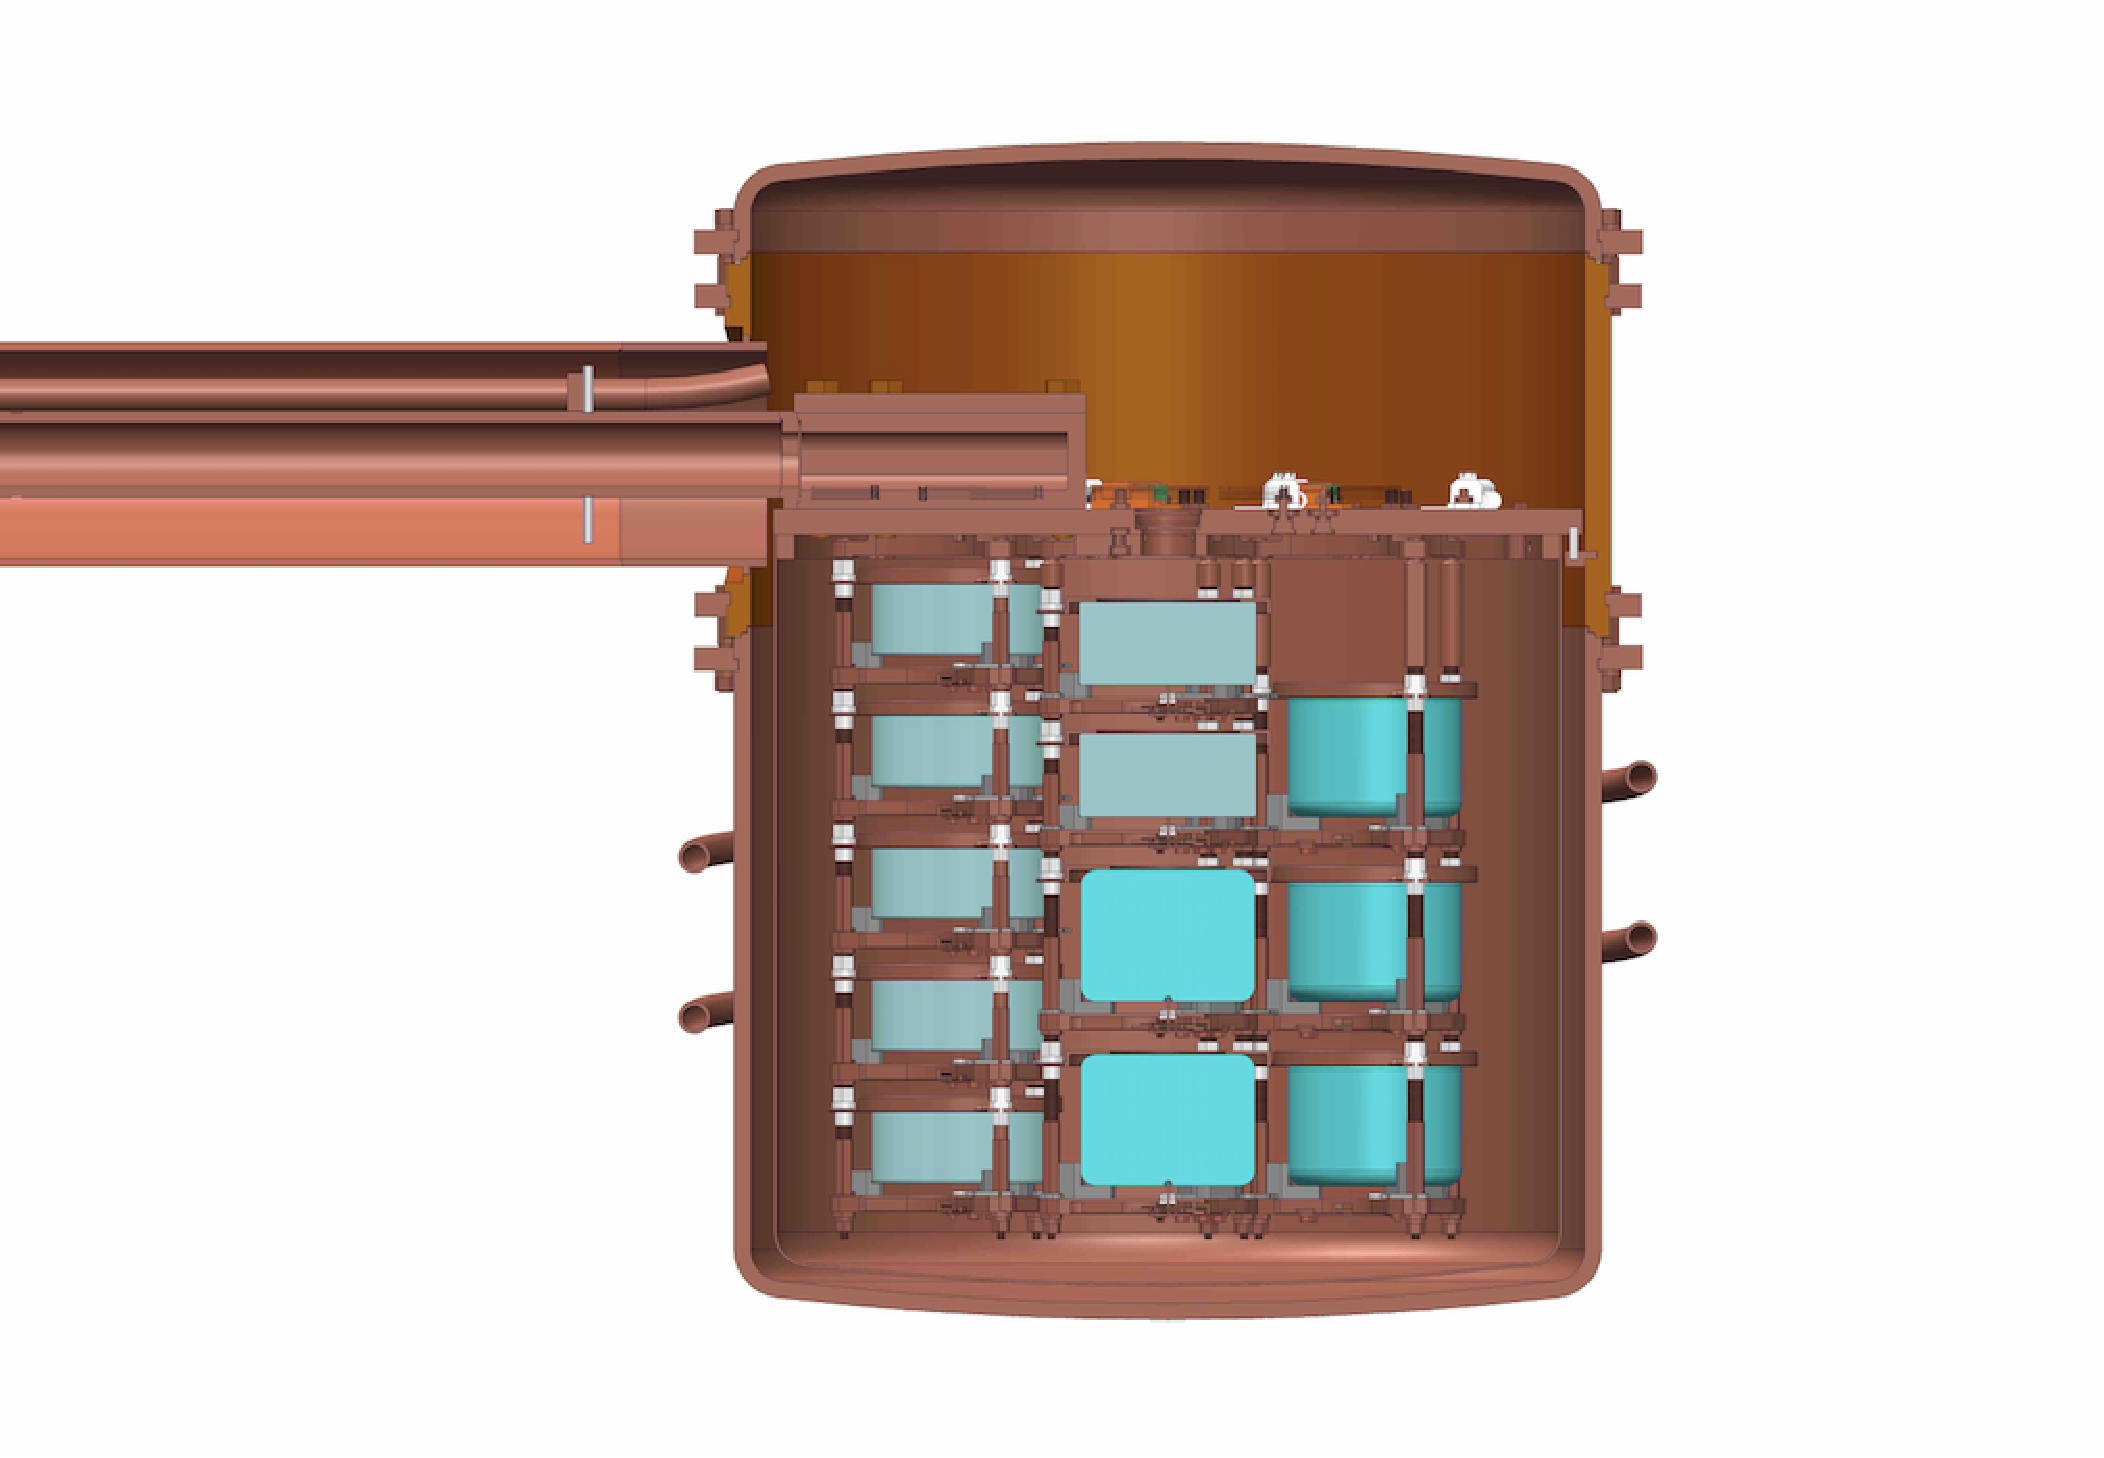
\includegraphics[width=0.7\textwidth]{/Users/cbartram/Downloads/example_diss/1_introduction/figures/mjd_cryostat.pdf}
\caption[%
\textsc{Majorana Demonstrator} cryostat drawing
]{%
Drawing of a \textsc{Majorana Demonstrator} cryostat. Strings of germanium crystals (turquoise) hang from the cryostat cold plate.
\label{fig:mjd_cryostat}} 
\end{figure}
% ------------  figure end 


%=====================%
\chapter{Simulation}
%=====================%
%-------------------------------------------------------------------%
\section{Geant Simulation}
%-------------------------------------------------------------------%

Using Geant4 [18], we have created a replica of the APEX geometry for our simulation. Most of the code
for the detector construction was written by Stephen Daigle. Some improvements have recently been made
by an undergraduate, Chiara Salemi, who is working with our group. We have added additional components
to the simulation, specically the electromagnet and a holder containing the source and aerogel. I have
implemented one possible source holder in the simulation (Figure 11), complete with the positron source
(22Na) deposited on kapton foil and sandwiched between pieces of scintillator and aerogel. In the simulation,
as in the physical world, a positron exiting the source is tagged and then scatters within the aerogel until
it loses enough kinetic energy to form positronium. The aluminium source and all of its constituents were
incorporated into the simulation this past year.


%-------------------------------------------------------------------%
\section{Another Section}
\label{sec:mjd}
%-------------------------------------------------------------------%
 \section{Experimental Setup}

\subsection{Positronium Formation, Decay, and Detection}

Our experiment can be conceptualized by visualizing the trajectory of a positron which originates in the center of the array and mentally tracking its subsequent interactions. The positron is emitted from a $\mathrm{{}^{22}Na}$ source in the middle of our detector. $\mathrm{{}^{22}Na}$ decays via the emission of a beta particle (Figure 10) to an excited state of $\mathrm{{}^{22}Ne}$, with a $90\%$ branching ratio. This state is short-lived and decays to the ground state of the $\mathrm{{}^{22}Ne}$ via emission of a 1.274 MeV gamma ray. Because the lifetime of the excited state is so short, the 1.274 MeV gamma ray can be used in the event selection process. 

Figure 5 shows a schematic of the proposed experiment. The $\mathrm{{}^{22}{Na}}$ is deposited on two thin sheets of kapton foil and sandwiched between scintillator. The scintillator, which is orthogonal to the $z$-axis of our cylindrical detector, tags the positron as it leaves the source. An optical fiber fed through a small hole in the source holder propagates the scintillation light to a nearby photomultiplier tube. This is the ``start signal'' for an event. The entire source holder is designed to be suspended in the center of the experiment via two long, hollow rods which fit into bore holes in the electromagnet.

Still in the source holder, the positron exits the scintillator and into an adjacent disk of aerogel. Aerogel is comprised of silica dioxide chains folded in such a way that the resulting material is highly porous. The aerogel borders the scintillator on both sides. Once the positron loses nearly all of its energy via scattering, it interacts with an electron in the $\mathrm{SiO_{2}}$ to form positronium. The positronium travels almost freely in the interstitial spaces of the aerogel until it decays, minimizing matter-interaction effects. The average lifetime of the $m=0$ states of positronium ($\sim$22 ns) is dictated by the 5 kGauss (0.5 T) magnetic field generated by our C-shaped electromagnet. We selected this field strength based on the optimum fields determined by previous groups. We will likely adjust this field strength as our studies of systematics mature. The electromagnet serves the dual purpose of separating our the spin states of ortho-positronium and providing spin-alignment. Based on the modeling described below, we have determined that our field inhomogeneity will be less than $2\%$, a significant improvement over the $10\%$ inhomogeneity of past experiments. Furthermore, we have the ability to switch the magnet's polarity, which will further reduce our systematics. This improvement has been suggested but not implemented by those who worked on previous $CP$-violating searches in positronium. The magnet is tapered in such a way that it cannot interfere with the trajectory of any positronium gamma ray which could be counted in our detector.

Gamma rays from the positronium decay propagate outwards, leaving the source holder and eventually reaching the sodium iodide segments of our detector, where they interact via the photoelectric effect and compton scattering. We use the APEX (ATLAS Positron Experiment~\cite{Mercer1994491}) array, a detector which consists of 24 trapezoidal sodium iodide segments (Figure 6). The dimensions of each segment is $\mathrm{55{\times}6{\times}5.5(7.0)\,cm^3}$. Each sodium iodide bar is bookended by two photomultiplier tubes, which pick up the resulting scintillation light in the crystal. The photomultiplier tubes run to the DAQ, situated in an electronics rack. Both the APEX detector and the electronics already exist at TUNL. 

 The cross section of the experiment is shown below.
 \begin{figure}[H]
 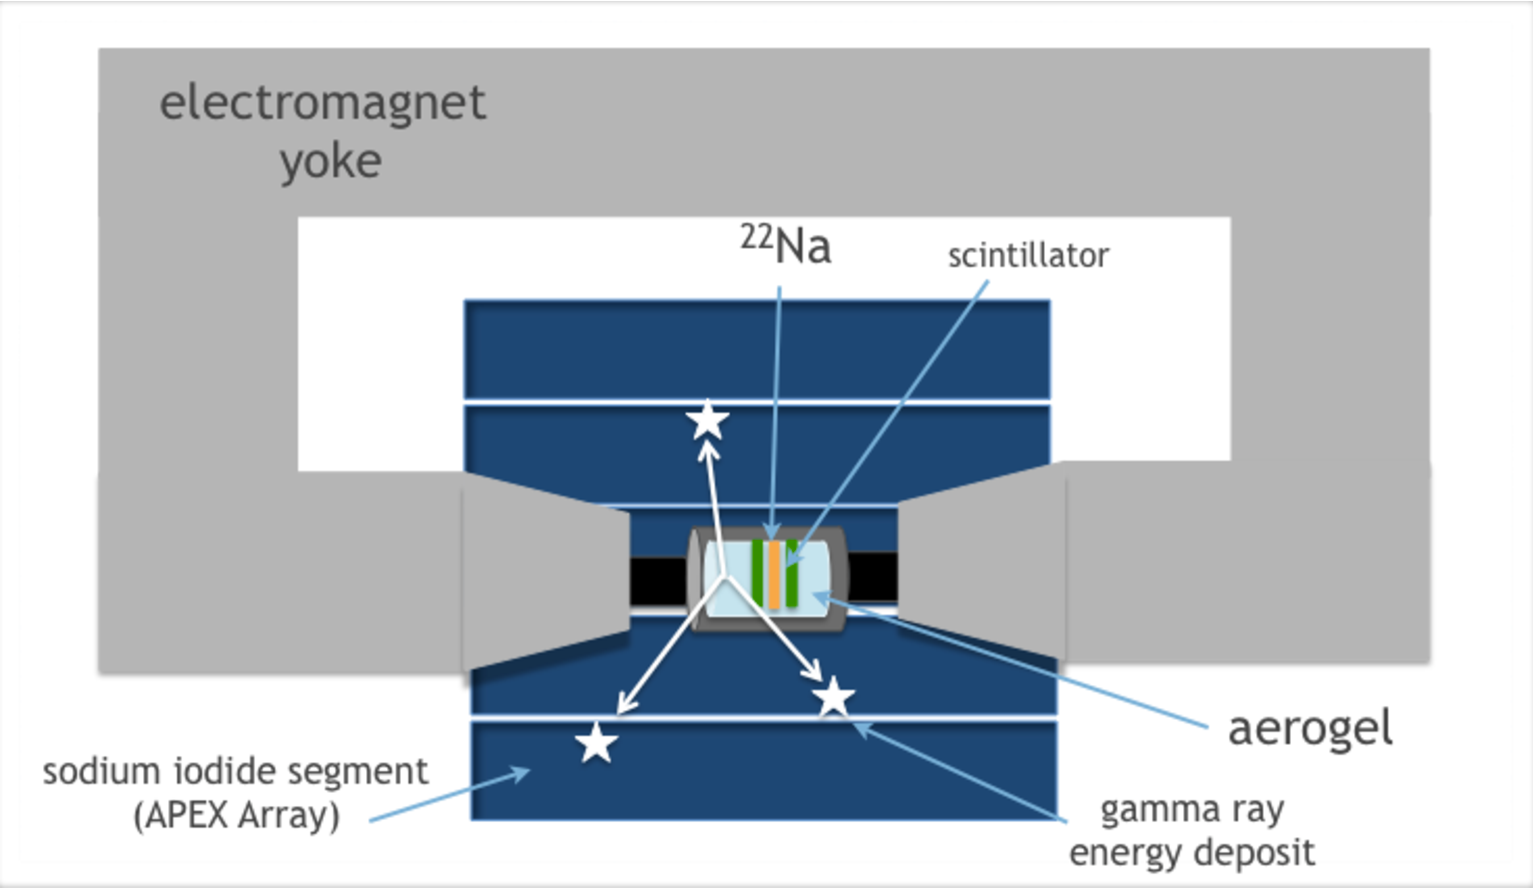
\includegraphics[width=0.75\textwidth,center]{CALIOPE_CrossSec.pdf}
 \caption{CALIOPE Cross Section (Bird's Eye View)}
 \end{figure}


\begin{wrapfigure}{r}{0.34\textwidth}
 \vspace{-10pt}
  \begin{center}
    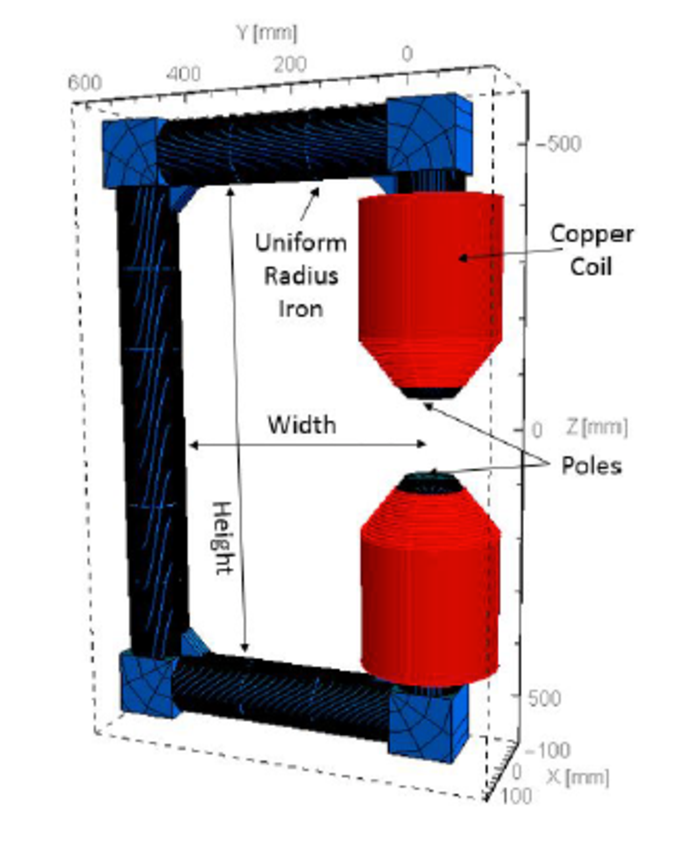
\includegraphics[width=0.34\textwidth]{Magnet.pdf}
  \end{center}
 \vspace{-10pt}
  \caption{Magnet}
\end{wrapfigure}

\subsection{Event Reconstruction}
 We calculate the position and energy of the hits in our detector by using the charge amplitudes measured by the photomultiplier tubes and a technique developed by a former graduate student, Stephen Daigle~\cite{StephenDaigle}. The amplitude of the signal from the first photomultiplier tube is
 \begin{align}
   A_{1}=\frac{E_{\gamma}P}{E_{0}}\exp[-\mu(L/2+z)]
 \end{align}
 where $z$ is the position of a hit, $E_{\gamma}$ is the energy deposited by the gamma ray, $P$ is the quantum efficiency of the photomultiplier tubes, $E_{0}$ is the energy deposited per light photon created in the scintillator and $\mu$ is the light attenuation coefficient. The attenuation coefficients were all measured by Stephen Daigle~\cite{StephenDaigle}. For the second photomultiplier tube, we have a similar equation:
 \begin{align}
 A_{2}=\frac{E_{\gamma}P}{E_{0}}\exp[-\mu(L/2-z)]
 \end{align}
 We can combine these equations to find the position in the bar from the charge amplitudes.
\begin{align}
 &z=\frac{1}{2\mu}\ln\frac{A_{2}}{A_{1}}
 \end{align}
 The resolution for the $z$ position was measured to be 3.5 cm FWHM.
 In a similar manner, the energy can also be calculated from the charge amplitudes using the following equation:
 \begin{align}
 &{E_{\gamma}}^{2}=A_{1}A_{2}\left(\frac{E_{0}}{P}\right)^2e^{{\mu}L} \\
 &E_{\gamma}=\sqrt{A_{1}A_{2}}\frac{E_{0}}{P}e^{{\mu}L/2}
 \end{align}

%\begingroup
%\setlength{\intextsep}{3pt}%
%\setlength{\columnsep}{3pt}%
% \begin{wrapfigure}{l}{0.32\textwidth}
% \vspace{-10pt}
%   \begin{center}
 %    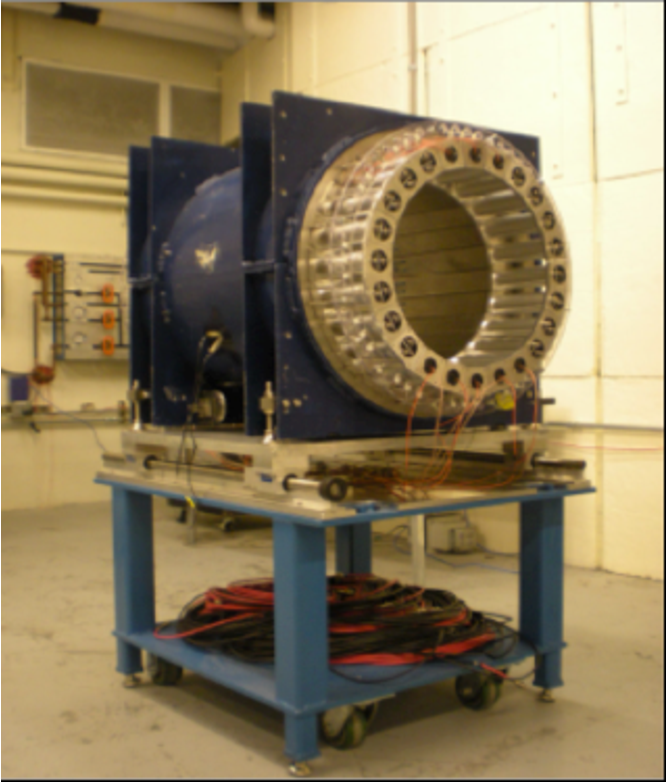
\includegraphics[width=0.32\textwidth]{APEX_Array.pdf}
 %  \end{center}
 %\vspace{-10pt}
 %  \caption{APEX Array at TUNL}
 %\end{wrapfigure}
%\endgroup


 \begin{figure}[!htb]
     \centering
     \begin{minipage}{.5\textwidth}
         \centering
         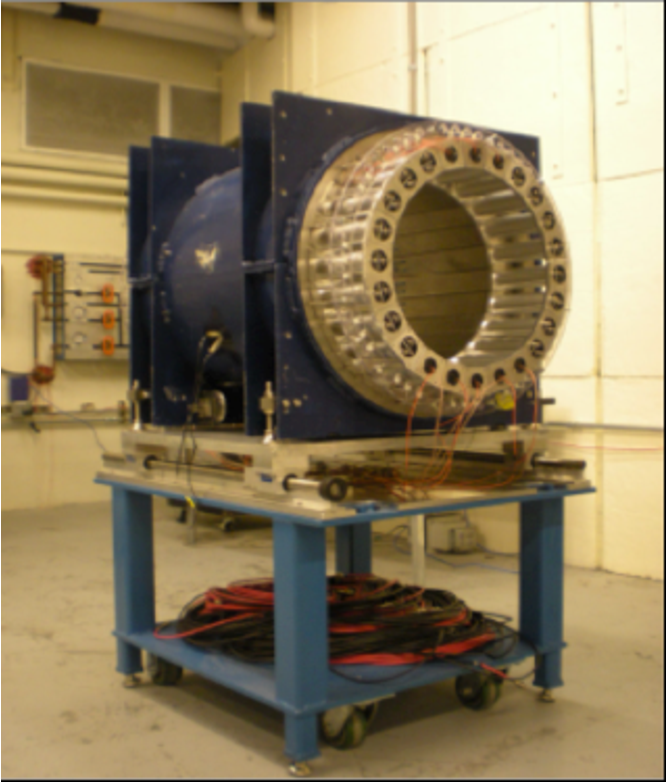
\includegraphics[width=0.6\linewidth]{APEX_Array.pdf}
         \caption{Side View of APEX at TUNL}
     \end{minipage}%                                                                                                                                                     
     \begin{minipage}{0.5\textwidth}
       \centering
       \includegraphics[width=0.7\linewidth]{APEX_Center.pdf}
       \caption{Front View of APEX at TUNL}
     \end{minipage}
 \end{figure}

 The resolution for the energy was measured to be 15\% for the 662 keV gamma ray line in $\mathrm{{}^{137}{Cs}}$. The large solid-angle coverage (75\%) and high intrinsic efficiency result in a total photopeak detection probability of 17\% at 1332 keV, as measured by Perry et al~\cite{2003NIMPA.505...85P}. 

 \begin{figure}[H]
 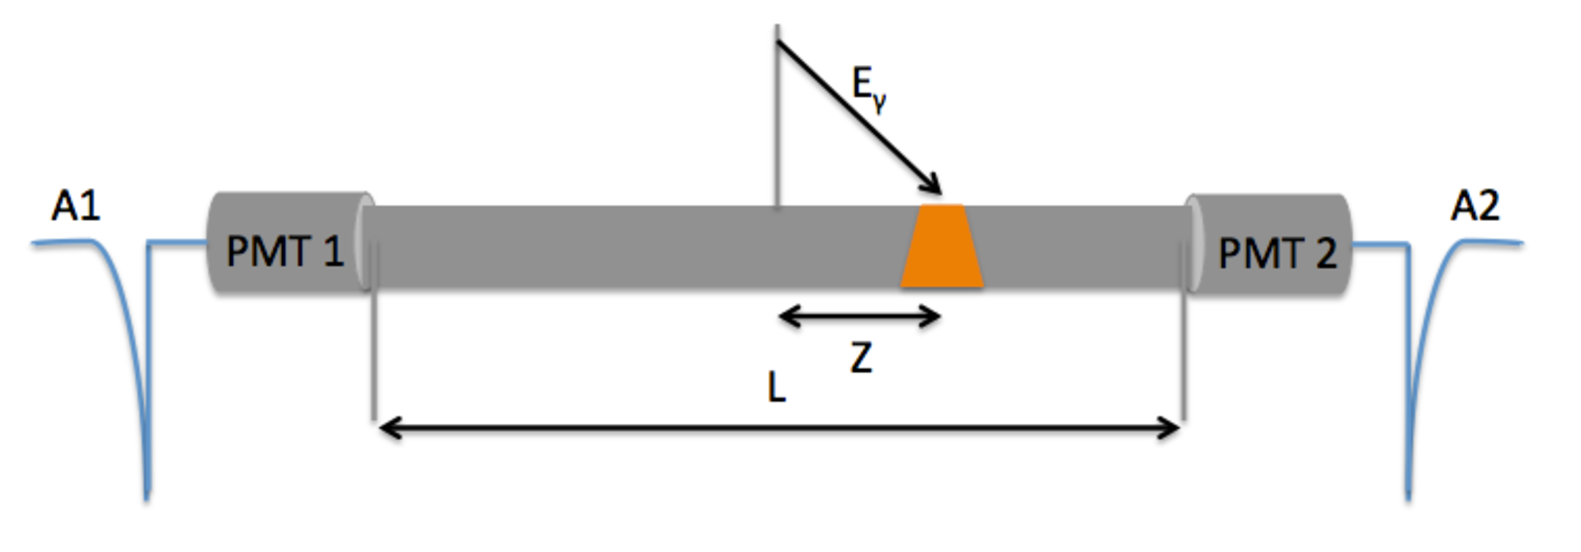
\includegraphics[width=0.7\textwidth,center]{NaI_Bar.pdf}
 \caption{NaI Segment}
 \end{figure}

This concludes our overview of the CALIOPE experiment. In the following section, we once again work from the inside out to present our experimental progress. We describe all facets of the construction, from the design phase up to the commissioning and integration of all major components of the experiment.


% ------------  figure start  
% from M. Busch
\begin{figure}[htbp]
\centering
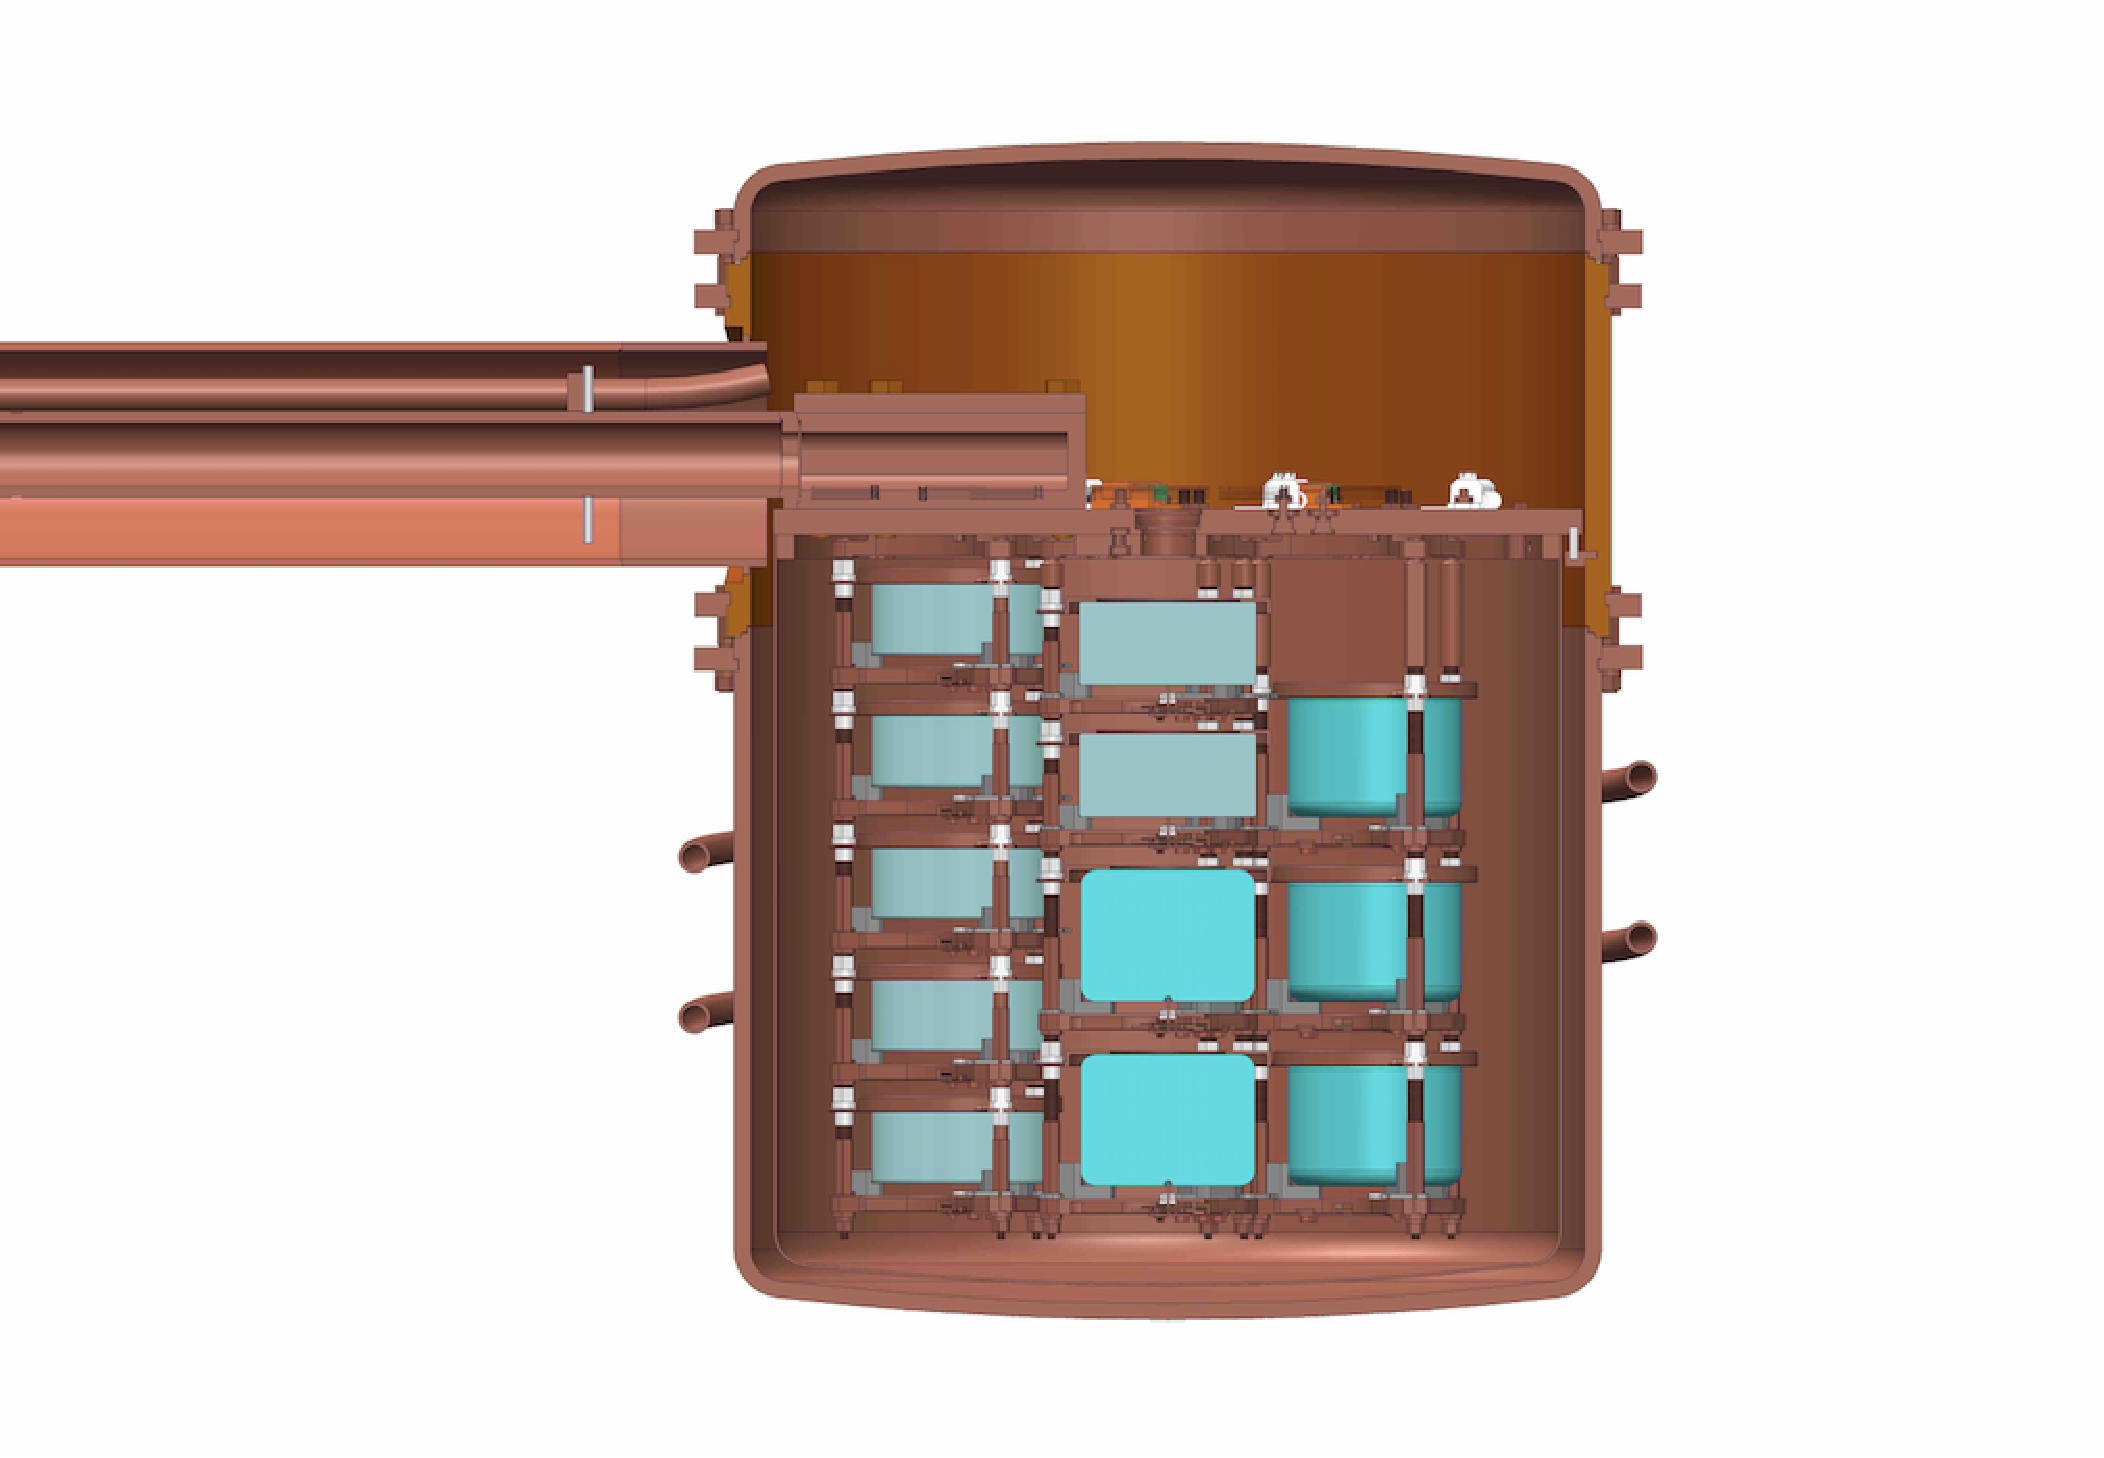
\includegraphics[width=0.7\textwidth]{/Users/cbartram/Downloads/example_diss/1_introduction/figures/mjd_cryostat.pdf}
\caption[%
\textsc{Majorana Demonstrator} cryostat drawing
]{%
Drawing of a \textsc{Majorana Demonstrator} cryostat. Strings of germanium crystals (turquoise) hang from the cryostat cold plate.
\label{fig:mjd_cryostat}} 
\end{figure}
% ------------  figure end 



\bibliographystyle{utcaps}
\bibliography{./gkg_dissertation}

\end{document}
